\documentclass[a4paper]{article}
\usepackage{mathtools}
\usepackage{pdfpages}
\usepackage{graphicx}
\usepackage{geometry}

\geometry{
  a4paper,
  total={170mm,257mm},
  left=20mm,
  top=20mm,
}

\title{Project B}
\author{Tung Pham}
\date{\today}

\begin{document}
\maketitle

\section{Part 1}
\subsection{Question 1a}
\begin{figure}[h]
	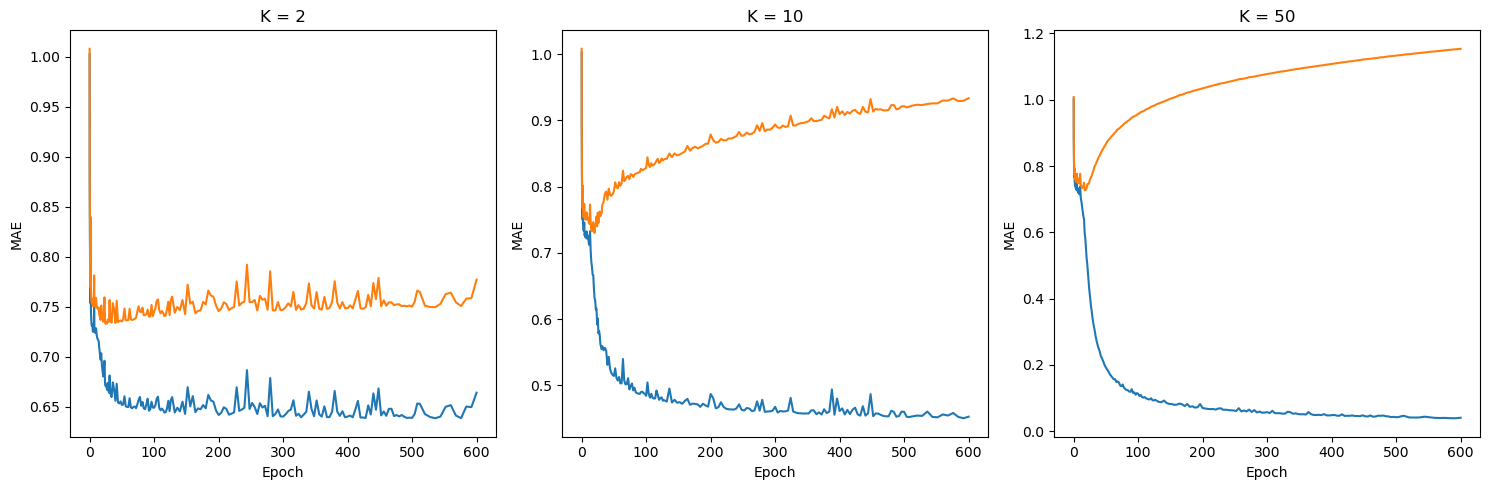
\includegraphics[width=\textwidth]{../images/Figure1a.png}
	\caption{All the graphs at first starts at a very high value of error. This is
  an indication of underfitting as the model has not yet been able to learned to
extract the pattern from the training data. As the number of epoch
increases, with SGD, we can see that the graphs of both training and validation
error began to converge. However, for all Ks, we can see that there is a sign of
overfitting as epochs go over 10. We can see that approximately at epoch 5, the
data began to converges and after 10, we can clearly see the separation between
training and validation error. Validation error went up while training error
went down significantly which indicates sign of overfitting of the model.}
\end{figure}
\subsection{Question 1b}
To select the best hyperparameters, we modified the SGD model for early stopping
and try out with different alphas, batch\_size and step\_size.

Below are the values that we've tried:
\begin{itemize}
  \item alphas: [0.0, 0.0001, 0.001, 0.1]
  \item batch\_sizes: [16, 32, 128, 1016]
  \item step\_sizes: [0.1, 0.3, 0.9, 2.7]
\end{itemize}

From 1a, we were able to see that most of the Ks values began to converges
around 200 epochs. Using this information, we began our search using epochs as
200. Using alpha as 0, we conduct hyperparameters search as seen below:

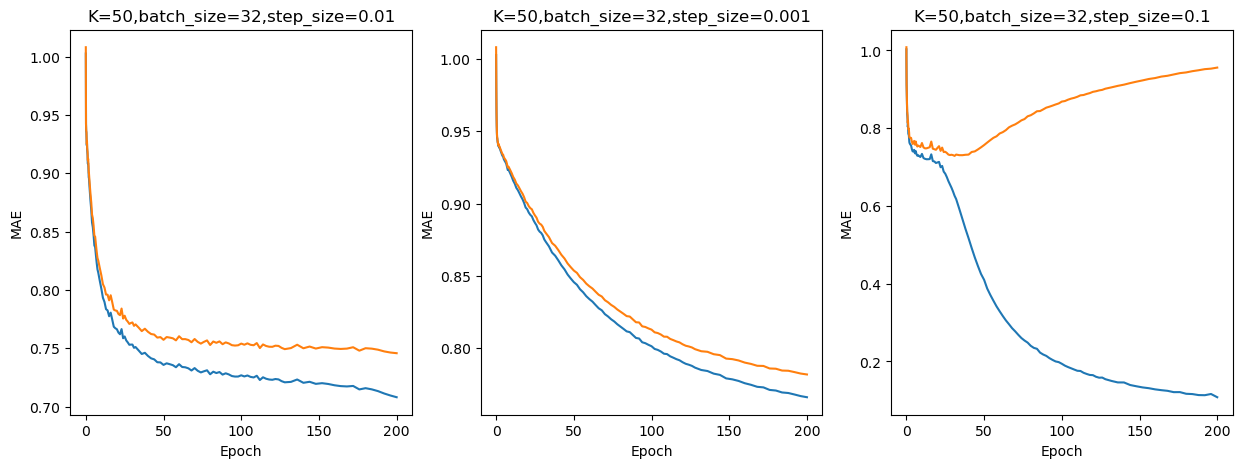
\includegraphics[width=\textwidth]{../images/1b-k50-bs32.png}

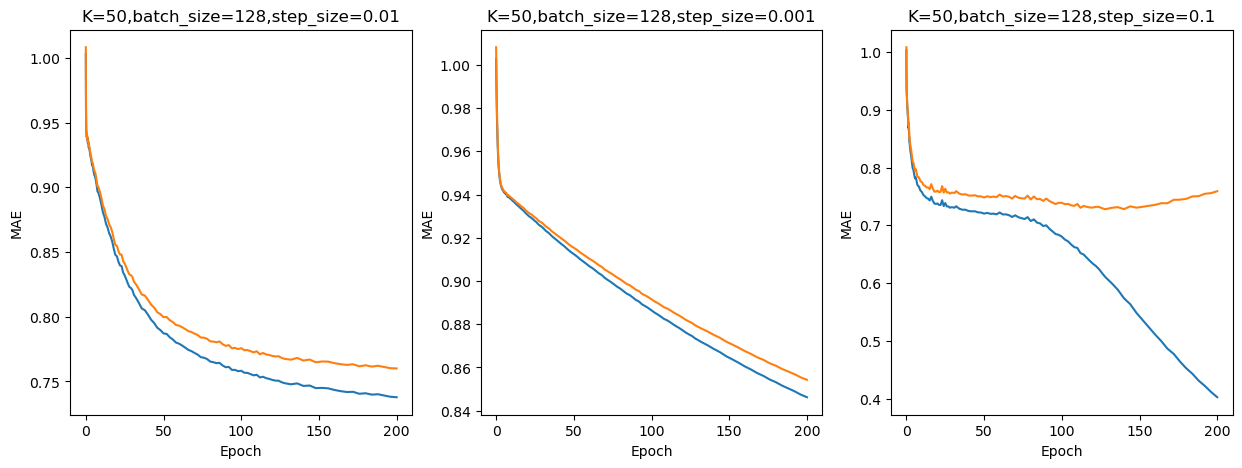
\includegraphics[width=\textwidth]{../images/1b-k50-bs128.png}

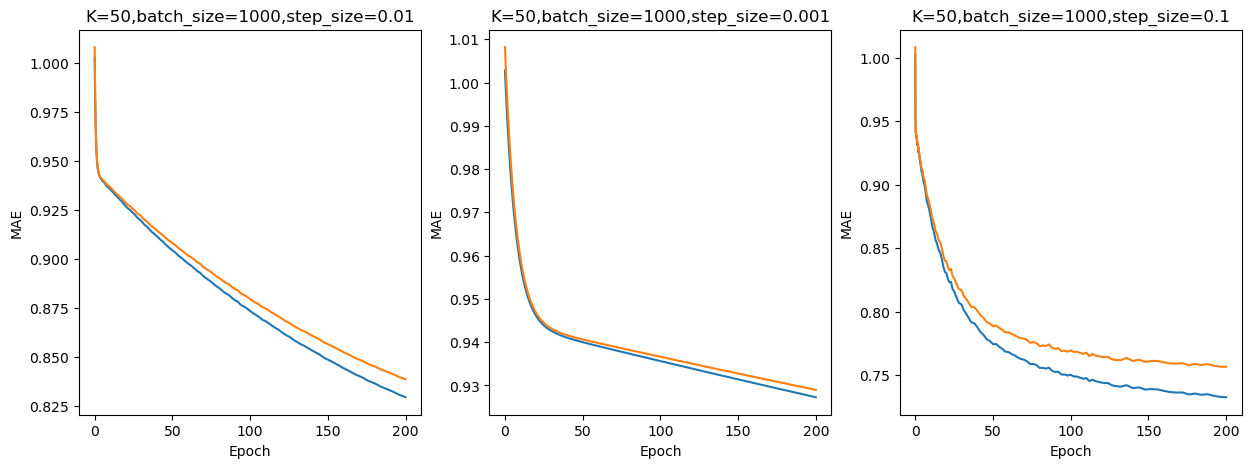
\includegraphics[width=\textwidth]{../images/1b-k50-bs1000.png}

With batch\_size of 1000 and step\_size of 0.1, we can see that it comes with
fast convergences in comparison to all other hyperparameters and able to achieve
the lowest training and validation errors. As for batch\_size of 32 and
step\_size 0.01, it's true that the combination provides fast convergences,
however, due to low batch_size, the graph is not smooth + we can see signs of
overfitting when it's reaching 200 epochs.

\begin{figure}[h]
	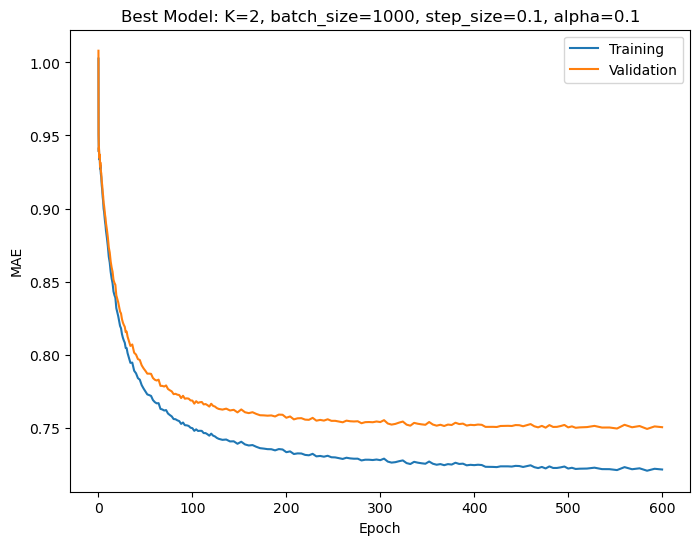
\includegraphics[width=\textwidth]{../images/Figure1b.png}
	\caption{For the best hyperparameters that achieved the best held out error,
  we were concluded that amongs the test values, alpha = 0.1, step\_size=0.1 and
batch\_size=1000 were able to achieves the lowest error on the heldout set. This
held out value was better than K=50 with 0.0 alpha }
\subsection{Question 1c}
To select the best values for hyperparameters batch\_size, step\_size and alpha,
we began exploring the possible batch\_sizes again.

\section{Part 2}
\subsection{Question 2a}

\end{figure}
\end{document}


